\section{Memory Transaction Optimization}
\label{sec:strategies} In this section, we elaborate on our two optimization algorithms. The key idea is to reduce the  number of memory
transactions which leads to the improvement in performance. Based on the observations shown in Figure \ref{fig:twostrategies}, we propose
two reuse algorithms, column reuse and row reuse, which can significantly reduce the number of memory transactions.


\subsection{Column Reuse}
\begin{figure*}
	\begin{subfigure}{0.33\textwidth}
		\centering
		\captionsetup{width=0.9\textwidth}
		 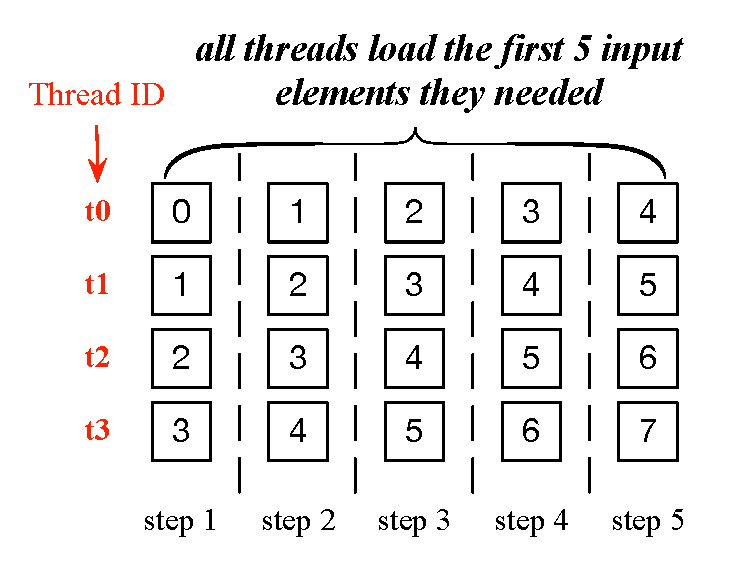
\includegraphics[width=0.98\textwidth,height=4.5cm]{./figure/directconv.eps}
		 \caption{Direct convolution: Each thread loads 5 input elements from global memory.}
		 \label{fig:directalgo}
	\end{subfigure}
	\begin{subfigure}{0.3\textwidth}
		\centering
		\captionsetup{width=0.9\textwidth}
		 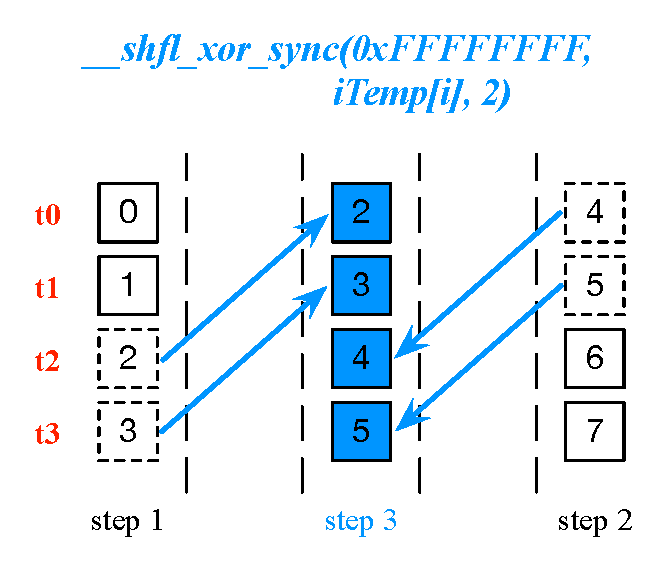
\includegraphics[width=\textwidth,height=4.5cm]{./figure/optalgo1.eps}
		 \caption{Optimized convolution: each thread retrieve its third element from the corresponding thread.}
		 \label{fig:optalgo1}
	\end{subfigure}
	\begin{subfigure}{0.3\textwidth}
		\centering
		\captionsetup{width=0.9\textwidth}

		 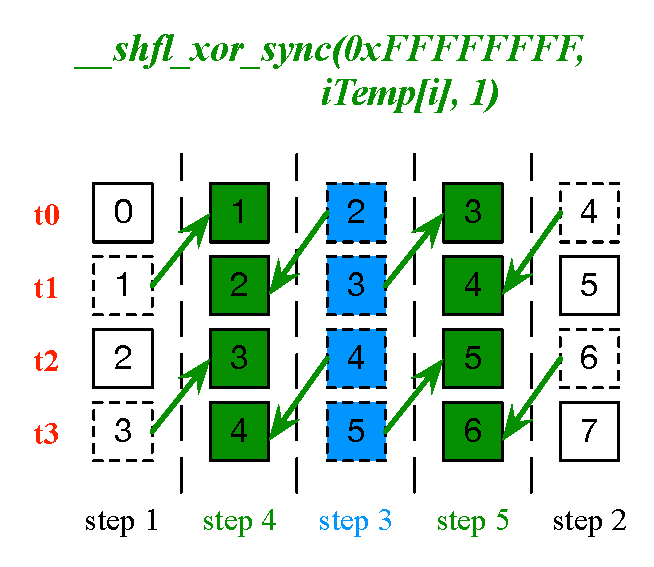
\includegraphics[width=0.96\textwidth,height=4.5cm]{./figure/optalgo2.eps}
		 \caption{Optimized convolution: each thread retrieve its second and fourth elements from corresponding threads.}
		 \label{fig:optalgo2}
	\end{subfigure}
  \caption{Illustration of direct and optimized convolution. We use a $5 \times 5$ filter  and each thread calculate convolution for one output element. Here we demonstrate how each thread processes first 5 corresponding input elements.}
   \label{fig:corealgo}
\end{figure*}

In this section, we demonstrate how to perform column reuse to eliminate duplicate columns. Using the convolution operation in Figure \ref{fig:twostrategies} as an example, we present the process of column reuse in Figure \ref{fig:corealgo}.%Each thread loads the first 5 corresponding input elements (each thread needs to load $F_H \times F_W \times F_C = 5 \times 5 \times 1 = 25$ input elements in total) to calculate the convolution of one output element.

\begin{figure}
	\centering
	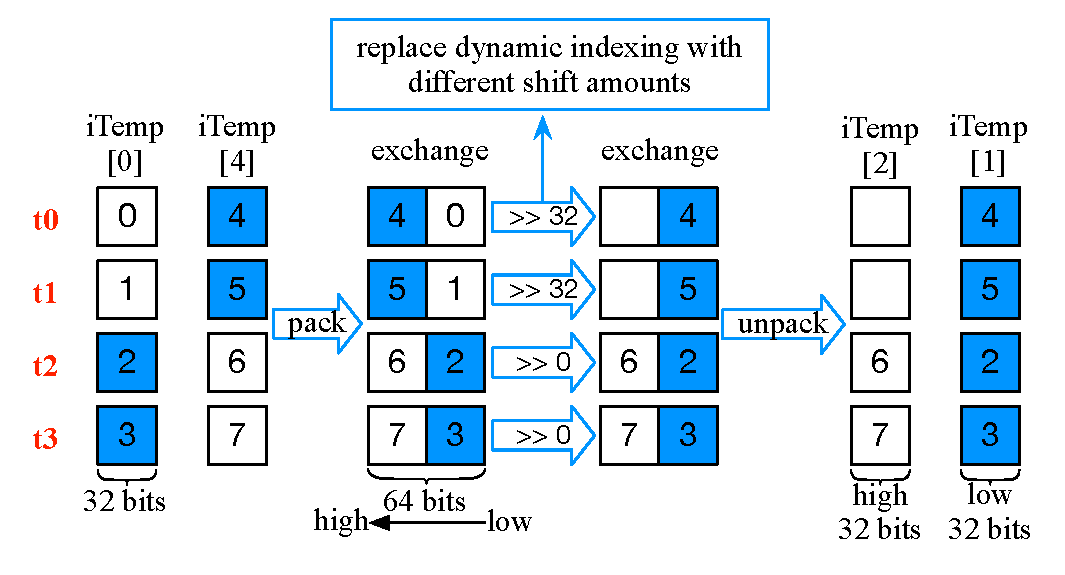
\includegraphics[width=\columnwidth,height=4.5cm]{./figure/exchange.eps}
\caption{Convert the dynamic indexing of array $iTemp$ into static indexing. Therefore, The compiler can put $iTemp$ into registers instead of local memory.}
\label{fig:exchange}
\end{figure}


In step 1 of Figure \ref{fig:directalgo}, each thread loads the first corresponding input elements from global memory. Because
addresses of these elements are contiguous (0, 1, 2, 3), the memory controler can coalesce these accesses into one memory transaction. Therefore, 5
memory transactions are required for step 1-5 of Figure \ref{fig:directalgo}. Each pair of adjacent threads have four duplicate input
elements, which corresponds to duplicate columns in Figure \ref{fig:twostrategies}. Next, we details how to eliminate this type of
duplication.

As we can see from Figure \ref{fig:directalgo}, input elements 1, 2, 3 loaded in step 2 are already loaded by thread $t1$, $t2$, $t3$ in
step 1. Therefore, we can retrieve input elements 1, 2, 3 from thread $t1$, $t2$, $t3$ instead of loading them from global memory (or L1
cache). This kind of duplication also occurs in step 3, 4, 5.

To eliminate redundant loads, we use shuffle instructions to exchange input elements among different threads. In step 1
and step 2 of Figure \ref{fig:optalgo1}, each thread loads its first and the fifth input elements from global memory. In step 3, each
thread utilizes shuffle instruction to retrieve its third element from another thread. Threads $t0$ and $t1$ retrieve their third elements
from threads $t2$ and $t3$ respectively, and also provide their fifth elements (shown as dashed square in step 2) for thread $t2$ and $t3$.
In the meantime, threads $t2$ and $t3$ retrieve their third elements from threads $t0$ and $t1$ respectively, and also provide their first
elements (shown as dashed square in step 1) for threads $t0$ and $t1$. This exchange process can be implemented using the instruction
$shfl\_xor(iTemp[i],2)$ (we take CUDA shuffle as an example, the exact form of shuffle instructions can be found at \cite{CUDAtoolkit}), where $iTemp$ is the thread local
array used to store five input elements and $i$ indexes which element to provide. For threads $t0$ and $t1$, both need to provide the fifth
elements, therefore $i=4$. For threads $t2$ and $t3$, both need to provide the first elements, therefore $i=0$. Figure \ref{fig:optalgo2}
has the similar procedure as Figure \ref{fig:optalgo1}, the difference is that each thread in Figure \ref{fig:optalgo2} retrieve its second
and fourth elements from its neighboring threads.


However, the instruction $shfl\_xor(iTemp[i],2)$ significantly degrades the performance of convolution. Because $iTemp$ is an array with
dynamic indexing, which means that the compiler can not decide which element to provide at compile time. Therefore the compiler will
place array $iTemp$ in local memory which has the same access latency as global memory, instead of registers. This will significantly
increase the memory access time and degrade the performance of convolution.

\begin{algorithm}
	$tid \gets threadIdx.x$\;
	$iTemp[0] \gets iData[iIndex]$\;
	$iTemp[4] \gets iData[iIndex+4]$\;
	$mov\ exchange, \{iTemp[0], iTemp[4]\}$\;
	$shift \gets ((tid+2)\&2)<<4$\;
	$exchange \gets exchange >> shift$\;
	$mov\ \{iTemp[1],iTemp[2]\}, exchange$\;
	$iTemp[2] \gets shfl\_xor(iTemp[1],2)$\;	
	
	\caption{Data exchange algorithm for retrieving the third element}
	\label{algo:basic}
\end{algorithm}

To convert dynamic indexing into static indexing, we design Algorithm \ref{algo:basic} for step 3 in Figure \ref{fig:optalgo1} and
Algorithm \ref{algo:basic2} for step 4 and 5 in Figure \ref{fig:optalgo2}. Both algorithms use the same method but deal with different
situations. Both algorithms can change dynamic indexing into static indexing and reduce the number of memory accesses. We use Algorithm
\ref{algo:basic} as an example to illustrate how to eliminate dynamic indexing.

Figure \ref{fig:exchange} illustrates the process of Line 4-7 of Algorithm \ref{algo:basic}. Each thread loads the first and fifth
corresponding input elements into thread local array $iTemp$ (Line 2-3). Then, pack both 32-bit elements into a 64-bit variable $exchange$
where $iTemp[4]$ is the high 32 bits and $iTemp[0]$ is the low 32 bits (Line 4). As threads $t0$ and $t1$ need to provide the their fifth
elements which are high 32 bits of $exchange$, we right shift $exchange$ by 32 to put $iTemp[4]$ in low 32 bits. For threads $t2$ and $t3$,
both need to provide their first elements which are already low 32 bits of $exchange$. therefore we right shift $exchange$ in threads $t2$
and $t3$ by 0. Shift amounts of each thread is calculated based on the thread id (Line 5). Afterwards, unpack $exchange$ into $iTemp[2]$
(high 32 bits) and $iTemp[1]$ (low 32 bits) (Line 7). And $iTemp[1]$ is the element that each thread needs to provide. Finally, using
shuffle instruction to exchange elements between threads (Line 8).

Compared with the previous usage of shuffle instruction \cite{vasilache2014fast}, Algorithm \ref{algo:basic} successfully replace dynamic
indexing $i$ in $shfl\_xor(iTemp[i],2)$ with static indexing $1$ in $shfl\_xor(iTemp[1],2)$. Algorithm \ref{algo:basic} successfully
eliminates dynamic indexing and therefore all thread local variables can be put in registers, which significantly improve the performance
of convolution.

\begin{algorithm}
	$tid \gets threadIdx.x$\;
	$mov\ exchange, \{iTemp[0], iTemp[2]\}$\;
	$shift \gets ((tid+1)\&1)<<5$\;
	$exchange \gets exchange >> shift$\;
	$mov\ \{iTemp[0],iTemp[1]\}, exchange$\;
	$iTemp[1] \gets shfl\_xor(iTemp[0],1)$\;	
	\caption{Data exchange algorithm for retrieving the second element}
	\label{algo:basic2}
\end{algorithm}

Step 4 and step 5 in Figure \ref{fig:optalgo2} have similar procedure as step 3 in Figure \ref{fig:optalgo1}. Thus, we slightly modify
Algorithm \ref{algo:basic} to obtain Algorithm \ref{algo:basic2}. The main distinction is that four threads are involved to exchange
elements in Figure \ref{fig:optalgo1} while only two adjacent threads are involved in Figure \ref{fig:optalgo2}. Accordingly, we need to
recalculate shift amounts for each thread (Line 3) and change arguments of the shuffle instruction (Line 6).

In summary, with Algorithm \ref{algo:basic} and \ref{algo:basic2}, we can reduce the number of memory transactions from 5 to 2 when loading
5 input elements and from 25 to 10 when loading 25 input elements. This reduction in the number of memory transactions brings a significant
performance improvements for convolution.

\subsection{Row Reuse}
\begin{figure}
	\centering
	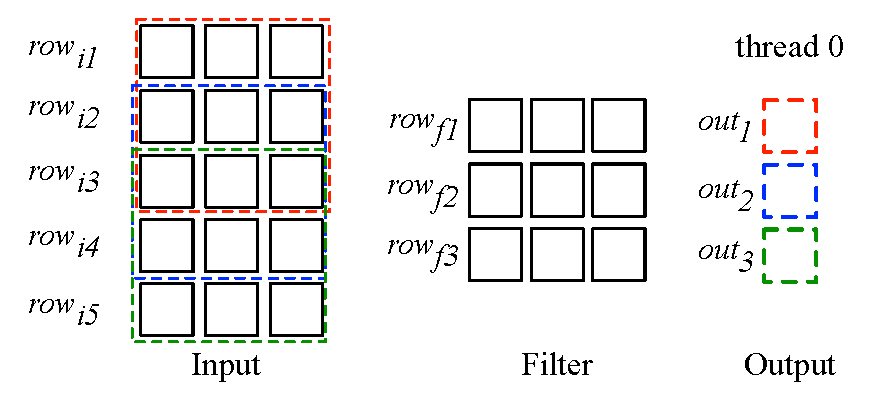
\includegraphics[width=\columnwidth,height=3.7cm]{./figure/rowreuse.eps}
\caption{A $3 \times 3$ filter is used to slide over the input image along height dimension and produce a column of output elements. One thread is used to calculate this column of output elements.}
\label{fig:rowreuse}
\end{figure}

When sliding the filter over the input image along height dimension, we can get a column of output elements, as shown in Figure
\ref{fig:rowreuse}. In our design, we use one thread to calculate one column of output elements. Based on Figure \ref{fig:rowreuse},
we can perform convolution as follows:

\begin{gather*}
  out_1=row_{i1} \cdot row_{f1} + row_{i2} \cdot row_{f2} + row_{i3} \cdot row_{f3} \\
out_{2}=row_{i2} \cdot row_{f1} + row_{i3} \cdot row_{f2} + row_{i4} \cdot row_{f3} \\
	out_{3}=row_{i3} \cdot row_{f1} + row_{i4} \cdot row_{f2} + row_{i5} \cdot row_{f3}
\end{gather*}

From above equations, we can see that $row_{i2}$ and $row_{i4}$ are loaded twice, $row_{i3}$ is loaded three times. We need to load 9 rows
in total. To eliminate row duplications, we redesign the way to perform convolution. After loading a row from input, we first determine how
many output elements need this row. For example, $row_{i1}$ is needed by $out_1$, $row_{i2}$ is needed by $out_1$ and $out_2$. Then, we use
this row to do inner product with corresponding rows of the filter to calculate output elements which need this row. Resigned formulations
are shown as follows:
\begin{equation}\nonumber
\begin{aligned}
load\ row_{i1}:
&\ out_1=row_{i1} \cdot row_{f1} \\
load\ row_{i2}:
&\ out_1 = out_1+row_{i2} \cdot row_{f2}\\
&\ out_2=row_{i2} \cdot row_{f1}\\
load\ row_{i3}:
&\ out_1 = out_1+row_{i3} \cdot row_{f3}\\
&\ out_2 = out_2+row_{i3} \cdot row_{f2}\\
&\ out_{3}=row_{i3} \cdot row_{f1}\\
load\ row_{i4}:
&\ out_2=out_2+row_{i4} \cdot row_{f3} \\
&\ out_3=out_3+row_{i4} \cdot row_{f2}\\
load\ row_{i5}:
&\ out_3=out_3+row_{i5} \cdot row_{f3}
\end{aligned}	
\end{equation}



We can see from above equations that only 5 rows are loaded to calculate output elements. A more generalized description of the method is
shown in Algorithm \ref{algo:rowreuse}, $row$ denotes the row loaded from the input, $index$ denotes the index of $row$, $filter$ denotes
the vector of filter rows. Line 1-5 deals with the first $F_H-1$ rows ($row_{i1}$ and $row_{i2}$ in Figure \ref{algo:rowreuse}), these rows
are needed by less than $F_H$ output elements. Line 6-11 deals with rows that are needed by exactly $F_H$ output elements ($row_{i3}$ in
Figure \ref{algo:rowreuse}). Line 12-17 deals with last $F_H-1$ rows, these rows are needed by less than $F_H$ output elements ($row_{i4}$
and $row_{i5}$ in Figure \ref{algo:rowreuse}).

\begin{algorithm}
	\KwIn{$row$, $index$, $filter$, $Out$}
	\KwOut{$Out$}
	\If{$index \textless F_H-1$}{
		\For {$i \gets 0$ \KwTo $index+1$}{
			$Out[i] \gets Out[i]+row \cdot filter[index-i]$\;
		}
	}\ElseIf{$index \geq F_H-1$ \textbf{and} $index \textless I_H-F_H+1$}{
		\For {$i \gets 0$ \KwTo $F_H$}{
			$o_{index} \gets index-F_H+1+i$\;
			$Out[o_{index}] \gets Out[o_{index}]+row \cdot filter[F_H-1-i]$\;
		}
	}\Else{
		\For {$i \gets F_H-1$ \KwTo $0$}{
			$o_{index} \gets I_H-F_H+1$\;
			$Out[o_{index}] \gets Out[o_{index}]+row \cdot filter[F_H-i]$\;
		}
	}
	\caption{Row reuse}
	\label{algo:rowreuse}
\end{algorithm}

In summary, Algorithm \ref{algo:rowreuse} eliminates row duplications when sliding a filter over input along height dimension. The
algorithm loads each row of input exactly once and thus greatly reduces the number of memory transactions.
